\documentclass[../../relatorio.tex]{subfiles}
\begin{document}
Neste subsistema podem-se encontrar as funcionalidades relacionadas com os \textbf{Clientes} do sistema. 
Apesar de cada subsistema não estar intrinsecamente dependente de outros, estes não deixam de 
se relacionarem, como se pode verificar neste caso, com o \textbf{SSReparacoes}.

Este subsistema define todas as dinâmicas relativas aos clientes do Centro de Reparações e as suas interações, ao
nível do sistema desenvolvido, com as classes que engloba e as classes de outros subsistemas da arquitetura.

Encontram-se as classes principais:
\begin{itemize}
    \item Cliente
    \item Equipamento
\end{itemize}

\subsubsection{Cliente}
A classe cliente representa, como referido anteriormente, os clientes do centro de reparações. 
Estes possuem um ou mais equipamentos associados a sí, sendo que possuí um \textbf{Map} para os guardar, sendo a
chave o seu código de registo.
Adicionalmente têm associados a sí uma classe de \textbf{FormaContacto} para guardar os seus contactos, 
\textit{Email} e \textit{número}.

\subsubsection{Equipamento}
De um modo bidirecional, os equipamentos tem acesso aos seus proprietários, para facilitar a obtenção destes.
Adicionalmente ao seu identificador, código de registo e marca, o equipamento encontra-se associado ao um enum -
\textbf{EstadoEquipamento}, para parametrizar os vários estados do equipamento no decorrer da sua estadia no centro de 
reparações.
Como cada equipamento tem um histórico de reparações associado a ele, houve a necessidade de o equipamento estar relacionado 
com o subsistema \textbf{SSReparacoes} (Ver \ref{sec:ss_reparacoes}), na classe \textbf{Reparacao}.
Por necessidade esta relação é bidirecional, para permitir à reparação ter conhecimento do equipamente que está a reparar.

\subsubsection{GestClientesFacade}
Esta classe permite a gestão dos clientes e dos respetivos equipamentos associados, implementando a interface IGestClientes.
Esta classe possui todos os clientes e equipamentos do sistema.

Analisando os métodos que esta classe implementa, identificou-se que, para melhorar a navegabilidade
e a \textit{performance} do sistema, será necessário que este tenha um conjunto de atributos, nomeadamente:
\begin{itemize}
    \item[clientes]{Mapa de clientes que pode ser acessido através do seu identificador, nif}
    \item[equipamentos]{Mapa de equipamentos que pode ser acessido através do seu ID} 
\end{itemize}

\begin{figure}[!ht]
    \centering
    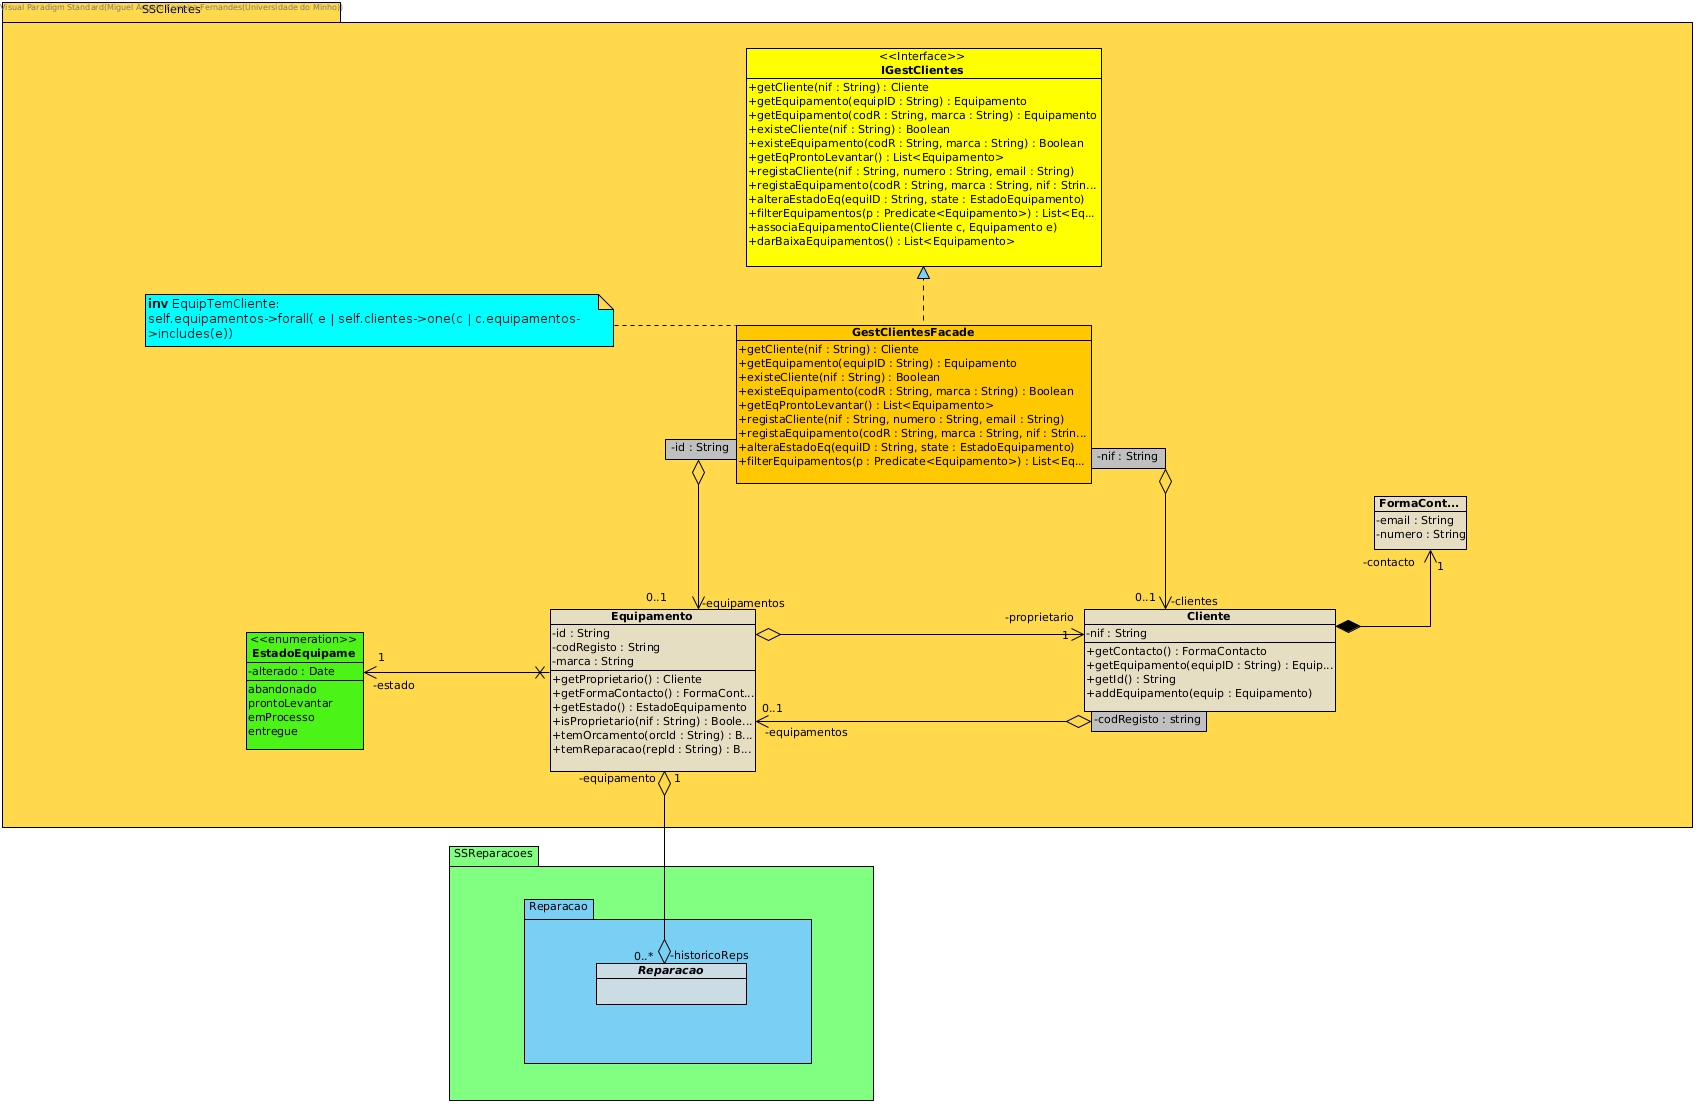
\includegraphics[scale=0.29]{SSClientes.jpg}
    \caption{SubSistema SSClientes \ref{sec:ss_clientes}}
\end{figure}
\end{document}